\documentclass{amsart}
\usepackage{amssymb,enumerate,bbm,amsmath}
\usepackage[colorlinks=true,linkcolor=blue,citecolor=blue]{hyper ref}
\usepackage{tikz}

\begin{document}

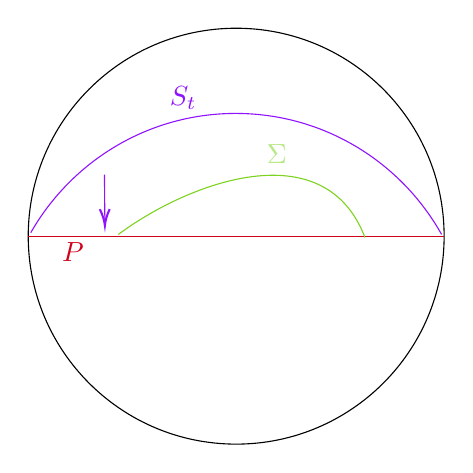
\begin{tikzpicture}[x=0.6pt,y=0.6pt,yscale=-0.9,xscale=0.9]
				
				\draw   (200,198.15) .. controls (200,121.3) and (262.3,59) .. (339.15,59) .. controls (416,59) and (478.3,121.3) .. (478.3,198.15) .. controls (478.3,275) and (416,337.3) .. (339.15,337.3) .. controls (262.3,337.3) and (200,275) .. (200,198.15) -- cycle ;
				\draw [color={rgb, 255:red, 208; green, 2; blue, 27 }  ,draw opacity=1 ]   (200,198.15) -- (478.3,198.15) ;
				\draw [color={rgb, 255:red, 126; green, 211; blue, 33 }  ,draw opacity=1 ]   (260.3,197) .. controls (307.3,162) and (398.3,128) .. (425.3,199) ;
				\draw  [draw opacity=0] (201.69,195.81) .. controls (229.21,147.67) and (281.11,115.46) .. (340.31,116.02) .. controls (398.91,116.57) and (449.76,149.1) .. (476.59,196.96) -- (338.81,274.75) -- cycle ; \draw  [color={rgb, 255:red, 144; green, 19; blue, 254 }  ,draw opacity=1 ] (201.69,195.81) .. controls (229.21,147.67) and (281.11,115.46) .. (340.31,116.02) .. controls (398.91,116.57) and (449.76,149.1) .. (476.59,196.96) ;  
				\draw [color={rgb, 255:red, 144; green, 19; blue, 254 }  ,draw opacity=1 ]   (251,157) -- (251.28,189) ;
				\draw [shift={(251.3,191)}, rotate = 269.49] [color={rgb, 255:red, 144; green, 19; blue, 254 }  ,draw opacity=1 ][line width=0.75]    (10.93,-3.29) .. controls (6.95,-1.4) and (3.31,-0.3) .. (0,0) .. controls (3.31,0.3) and (6.95,1.4) .. (10.93,3.29)   ;
				
				% Text Node
				\draw (358,135) node [anchor=north west][inner sep=0.75pt]  [color={rgb, 255:red, 126; green, 211; blue, 33 }  ,opacity=1 ] [align=left] {$\displaystyle \textcolor[rgb]{0.72,0.91,0.53}{\Sigma }$};
				% Text Node
				\draw (293,96.4) node [anchor=north west][inner sep=0.75pt]  [color={rgb, 255:red, 144; green, 19; blue, 254 }  ,opacity=1 ]  {$S_{t}$};
				% Text Node
				\draw (221,201) node [anchor=north west][inner sep=0.75pt]  [color={rgb, 255:red, 208; green, 2; blue, 27 }  ,opacity=1 ] [align=left] {$\displaystyle P$};
				
				
			\end{tikzpicture}

\end{document}